\documentclass[11pt]{article}
\usepackage[utf8]{inputenc}
\usepackage{graphicx}
\usepackage{float}
\title{Tsoha-Dokumentaatio}
\author{Ilmo Salmenperä}

\begin{document}
\maketitle
\newpage
\section{Johdanto}
Aktiivisena roolipelaaja ja pelinjohtajana itselläni on usein ongelmana muistiinpanojen säilyttäminen järkevässä paikassa, josta kaikki osapuolet voisivat lukea niitä kivuttomasti. Tarkoitus olisi luoda sivusto jossa olisi mahdollisuus pitää yllä useiden pelien muistiinpanoja järkevästi. 

Järjestelmässä kuka tahansa käyttääjä voi luoda pelin liittää siihen haluamiaan käyttäjiä pelaajia. Luodessaan sivun hänestä tulee tämän pelin pelinjohtaja. Hän voi luoda jokaiselle sessiolle oman sivunsa, jonne voi jälkikäteen kirjoittaa mitä pelissä on tapahtunut. Sen lisäksi pelinjohtaja voi tehdä yksittäisiä artikkeleita pelissä esiintyneistä asioista. Pelaajat voivat käydä lukemassa näitä, sekä hallinnoida omille hahmoillensa tehtyjä sivuja. Sivuja voi muuten lukea vapaasti, paitsi pelinjohtajalla on omia osioita jokaisella sivulla, joiden informaatio on piilossa kaikilta muilta paitsi tältä itseltään.

Järjestelmä on toteutettu PHP:n ja HTML:n avulla ja siinä on käytetty myös Twig sivupohjamoottoria, sekä Bootstrap websivusto frameworkkia. Järjestelmän pohjalla on Postgres-tietokanta, jonne kaikki järjestelmän tiedot talletetaan.

\section{Yleiskuva järjestelmästä}
Järjestelmän sisällä käyttäjiä ei erotella erikseen admineiksi, vaan jokaisen pelin pelinjohtajalla on aina enemmän valtuuksia pelin sisällä muihin järjestelmän käyttäjiin verrattuna. Tämän takia allaolevaan käyttötapauskaavioon on merkitty käyttäjä erikseen pelaajasta ja pelinjohtajasta. Pelinjohtajan ja pelaajan käyttötapaukset viittaavat pelin sisäisiin käyttötapauksiin ja käyttäjän käyttötapaukset viittavat pelien ulkopuoliseen toimintaan.

\begin{figure}[H]
\centering
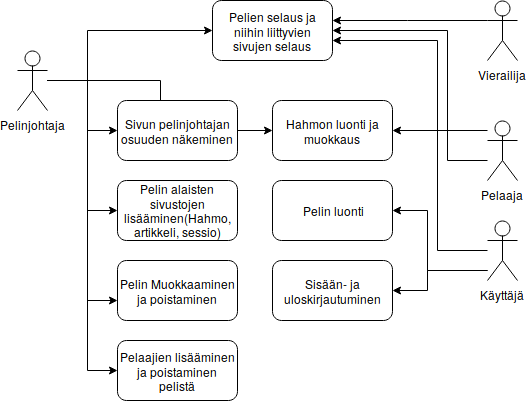
\includegraphics[scale=0.5]{pictures/kayttotapauskaavio.png}
\caption{Käyttötapauskaavio}
\end{figure}

\subsection{Käyttäjät}
Sivuston käyttäjät voidaan jakaa vierailijoihin, käyttäjiin, pelinjohtajiin ja pelaajiin.
\subsubsection{Vierailija}
Vierailija on rajoitetuin käyttäjä tyyppi. Tämä on kirjautumaton sivuston selaaja, joka voi ainoastaan lukea sivulle kirjoitettuja artikkeleja.

\subsubsection{Käyttäjä}
Käyttäjä pystyy kirjautumaan sisään ja pois järjestelmästä, sekä luoda oman pelinsä, jonka pelinjohtajaksi tämä pääsee. Käyttäjäryhmät pelaaja sekä pelinjohtaja ovat molemmat Käyttäjiä, mutta näiden käyttäjäryhmien muokkausoikeudet riippuvat siitä, ovatko nämä pelissä pelinjohtajia vai pelaajia.

\subsubsection{Pelaaja}
Pelaaja pystyy normaalin selauksen lisäksi luoda, poistaa sekä hallita oman hahmosa sivustoa.

\subsubsection{Pelinjohtaja}
Pelinjohtaja pystyy taas muokata oman pelinsä informaatiota tai jopa poistaa koko pelin. Hän pystyy lisätä, sekä poistaa pelistä pelaajia. Hän pystyy luomaan, muokkaamaan ja poistamaan pelin omalta sivulta artikkeleita, sessioita, sekä hahmoja. Hän pystyy lopuksi myös näkemään oman pelinsä pelinjohtajan osuuksia, jotka ovat kaikilta muilta käyttäjältä piilotettuja tekstiosuuksia.

\subsection{Käyttötapaukset}
Yleisiä käyttötapauksia ja niiden kuvauksia.

\subsubsection{Sivujen lukeminen}
Kuka tahansa pystyy käydä lukemassa minkä tahansa pelin tietoja pelinjohtajan osuuksia lukuunottamatta.

\subsubsection{Hahmon muokkaaminen}
Pelin hahmoja pystyy luoda, muokata tai poistaa joko kyseisen hahmon luonut pelaaja, tai koko pelin pelinjohtaja. 

\subsection{Artikkelien, pelien ja sessioiden muokkaaminen}
Pelin pelinjohtaja pystyy luoda, muokata ja poistaa peliin liittyviä sivuja vapaasti. 

\subsection{Pelaajien lisääminen ja poistaminen pelistä}
Pelinjohtaja pystyy lisätä ja poistaa käyttäjiä omaan peliinsä vapaasti. Poistaminen ei poista pelaajien hahmoja sivulta ja jos pelaaja lisätään takaisin, tällä pysyy oikeudet omaan hahmoonsa.

\subsubsection{Muita tapauksia}
Sivustolle kirjautuminen ja sieltä uloskirjautuminen.

\section{Järjestelmän tietosisältö}
Järjestelmässä on kuusi pääasiallista tietokohdetta, jotka ovat kuvattu alhaalla olevassa kaaviossa.
\begin{figure}[t]
\centering
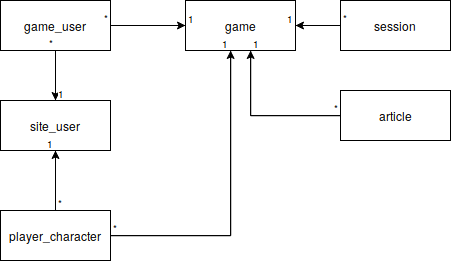
\includegraphics[scale=0.5]{pictures/kasitekaavio.png}
\caption{Käsitekaavio}
\end{figure}

\begin{figure}[H]
\caption{site\_user}
\begin{tabular}{| l | l | l |}
\hline
Atribuutti & Arvojoukko & Kuvailu \\
\hline
name & Merkkijono, max. 32 merkkiä & käyttäjän käyttäjätunnus \\
\hline
password & Merkkijono, max 64 merkkiä & käyttäjän salasana \\
\hline 
admin & boolean & admin tiedon antava jäänne suunnitteluvaiheesta. \\
 & & Ei käytetä tällä hetkellä mihinkkään \\
\hline
\end{tabular}
\end{figure}

\begin{figure}[H]
\caption{game}
\begin{tabular}{| l | l | l |}
\hline
Atribuutti & Arvojoukko & Kuvailu \\
\hline
name & Merkkijono, max. 64 merkkiä & Pelin nimi \\
\hline
system & Merkkijono, max 32 merkkiä & Pelin systeemi \\
\hline
description\_short & Merkkijono, max 128 & Lyhyt kuvaus pelistä etusivulle \\
\hline 
description & Merkkijono & Pitempi kuvaus pelistä pelin \\
& & omalle etusivulle \\
\hline
gm\_note & Merkkijono & Pelinjohtajan salaisia muistiinpanoja pelistä \\
\hline
\end{tabular}
\end{figure}

\begin{figure}[H]
\caption{game\_session}
\begin{tabular}{| l | l | l |}
\hline
Atribuutti & Arvojoukko & Kuvailu \\
\hline
name & Merkkijono, max. 64 merkkiä & Session nimi \\
\hline
description\_short & Merkkijono, max 128 & Lyhyt kuvaus sessiosta pelin etusivulle \\
\hline 
description & Merkkijono & Pitempi kuvaus sessiosta sen \\
& & omalle etusivulle \\
\hline
gm\_note & Merkkijono & Pelinjohtajan salaisia muistiinpanoja sessiosta \\
\hline
\end{tabular}
\end{figure}

\begin{figure}[H]
\caption{player\_character}
\begin{tabular}{| l | l | l |}
\hline
Atribuutti & Arvojoukko & Kuvailu \\
\hline
name & Merkkijono, max. 64 merkkiä & Hahmon nimi \\
\hline
description\_short & Merkkijono, max 128 & Lyhyt kuvaus hahmosta pelin etusivulle \\
\hline 
description & Merkkijono & Pitempi kuvaus hahmosta sen \\
& & omalle etusivulle \\
\hline
history & Merkkijono & Pelaajahahmon taustatarinaa \\
\hline
gm\_note & Merkkijono & Pelinjohtajan salaisia muistiinpanoja hahmosta \\
\hline
\end{tabular}
\end{figure}

\begin{figure}[H]
\caption{article}
\begin{tabular}{| l | l | l |}
\hline
Atribuutti & Arvojoukko & Kuvailu \\
\hline
name & Merkkijono, max. 64 merkkiä & Artikkelin nimi \\
\hline
description\_short & Merkkijono, max 128 & Lyhyt kuvaus artikkelista pelin etusivulle \\
\hline 
description & Merkkijono & Pitempi kuvaus artikkelista sen \\
& & omalle etusivulle \\
\hline
gm\_note & Merkkijono & Pelinjohtajan salaisia muistiinpanoja artikkelista \\
\hline
\end{tabular}
\end{figure}
\newpage
\section{Relaatiotietokantakaavio}
Alhaalla relaatiotietokantakaavio järjestelmästä.
\begin{figure}[H]
\centering
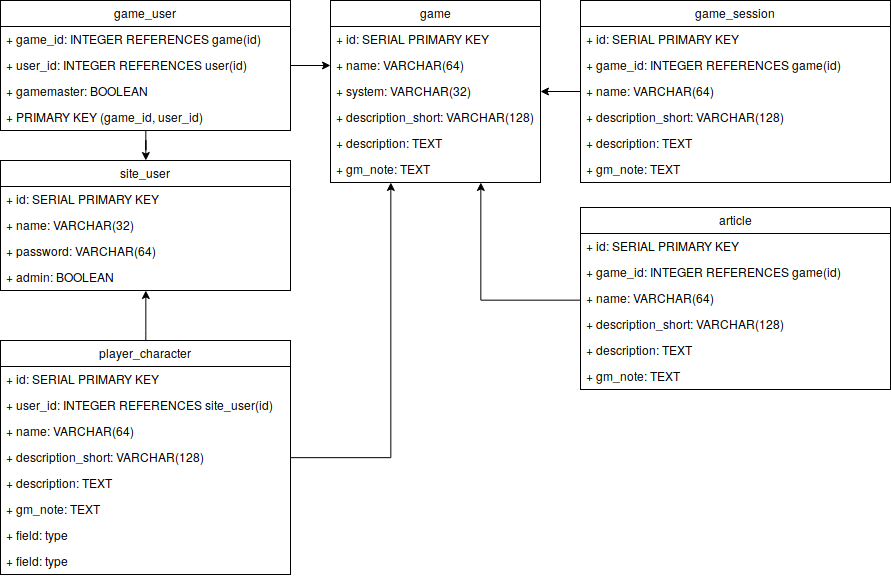
\includegraphics[scale=0.4]{pictures/relaatiokaavio.png}
\caption{Relaatiotietokantakaavio}
\end{figure}

\section{Järjestelmän yleisrakenne}
Tietokantasovellus noudattaa MVC-mallia. Kontrollerit, näkymät ja mallit sijaitsevat hakemistoissa controllers, views ja models. Apukirjastot sijaitsevat kansiossa lib ja asetukset tiedostossa settings.

\section{Asennustiedot}
Järjestelmän voi asentaa kopiomalla sen tiedostot palvelimen nettiin näkyvään hakemistoon. Sen jälkeen tietokannan yhteystiedot pitää kopioida oikein libs/config.php tiedostoon. Malli tähän löytyy tiedostosta libs/config.php.dist

\section{Käynnistys- ja käyttöohje}
Osoite löytyy asennettuna sivulta http://ilmosalm.users.cs.helsinki.fi/tsoha/. Sivulta löytyy neljä käyttäjää johtaja, pelaaja1, pelaaja2, pelaaja3. Johtajan salasana on johtaja ja jokaisen pelaaja käyttäjän salasana on pelaaja. 

\end{document}